\section{Results}
    In this section, we will present the results of all three experiments. In the heatmaps, the by red enclosed cells indicates the environments from the testing set used for extrapolation testing, while the non-red-enclosed cells represent the environments from the training set used for interpolation testing.
    \subsection{Experiment 1: One generalist}
        \begin{figure*}[ht]
            \centering
            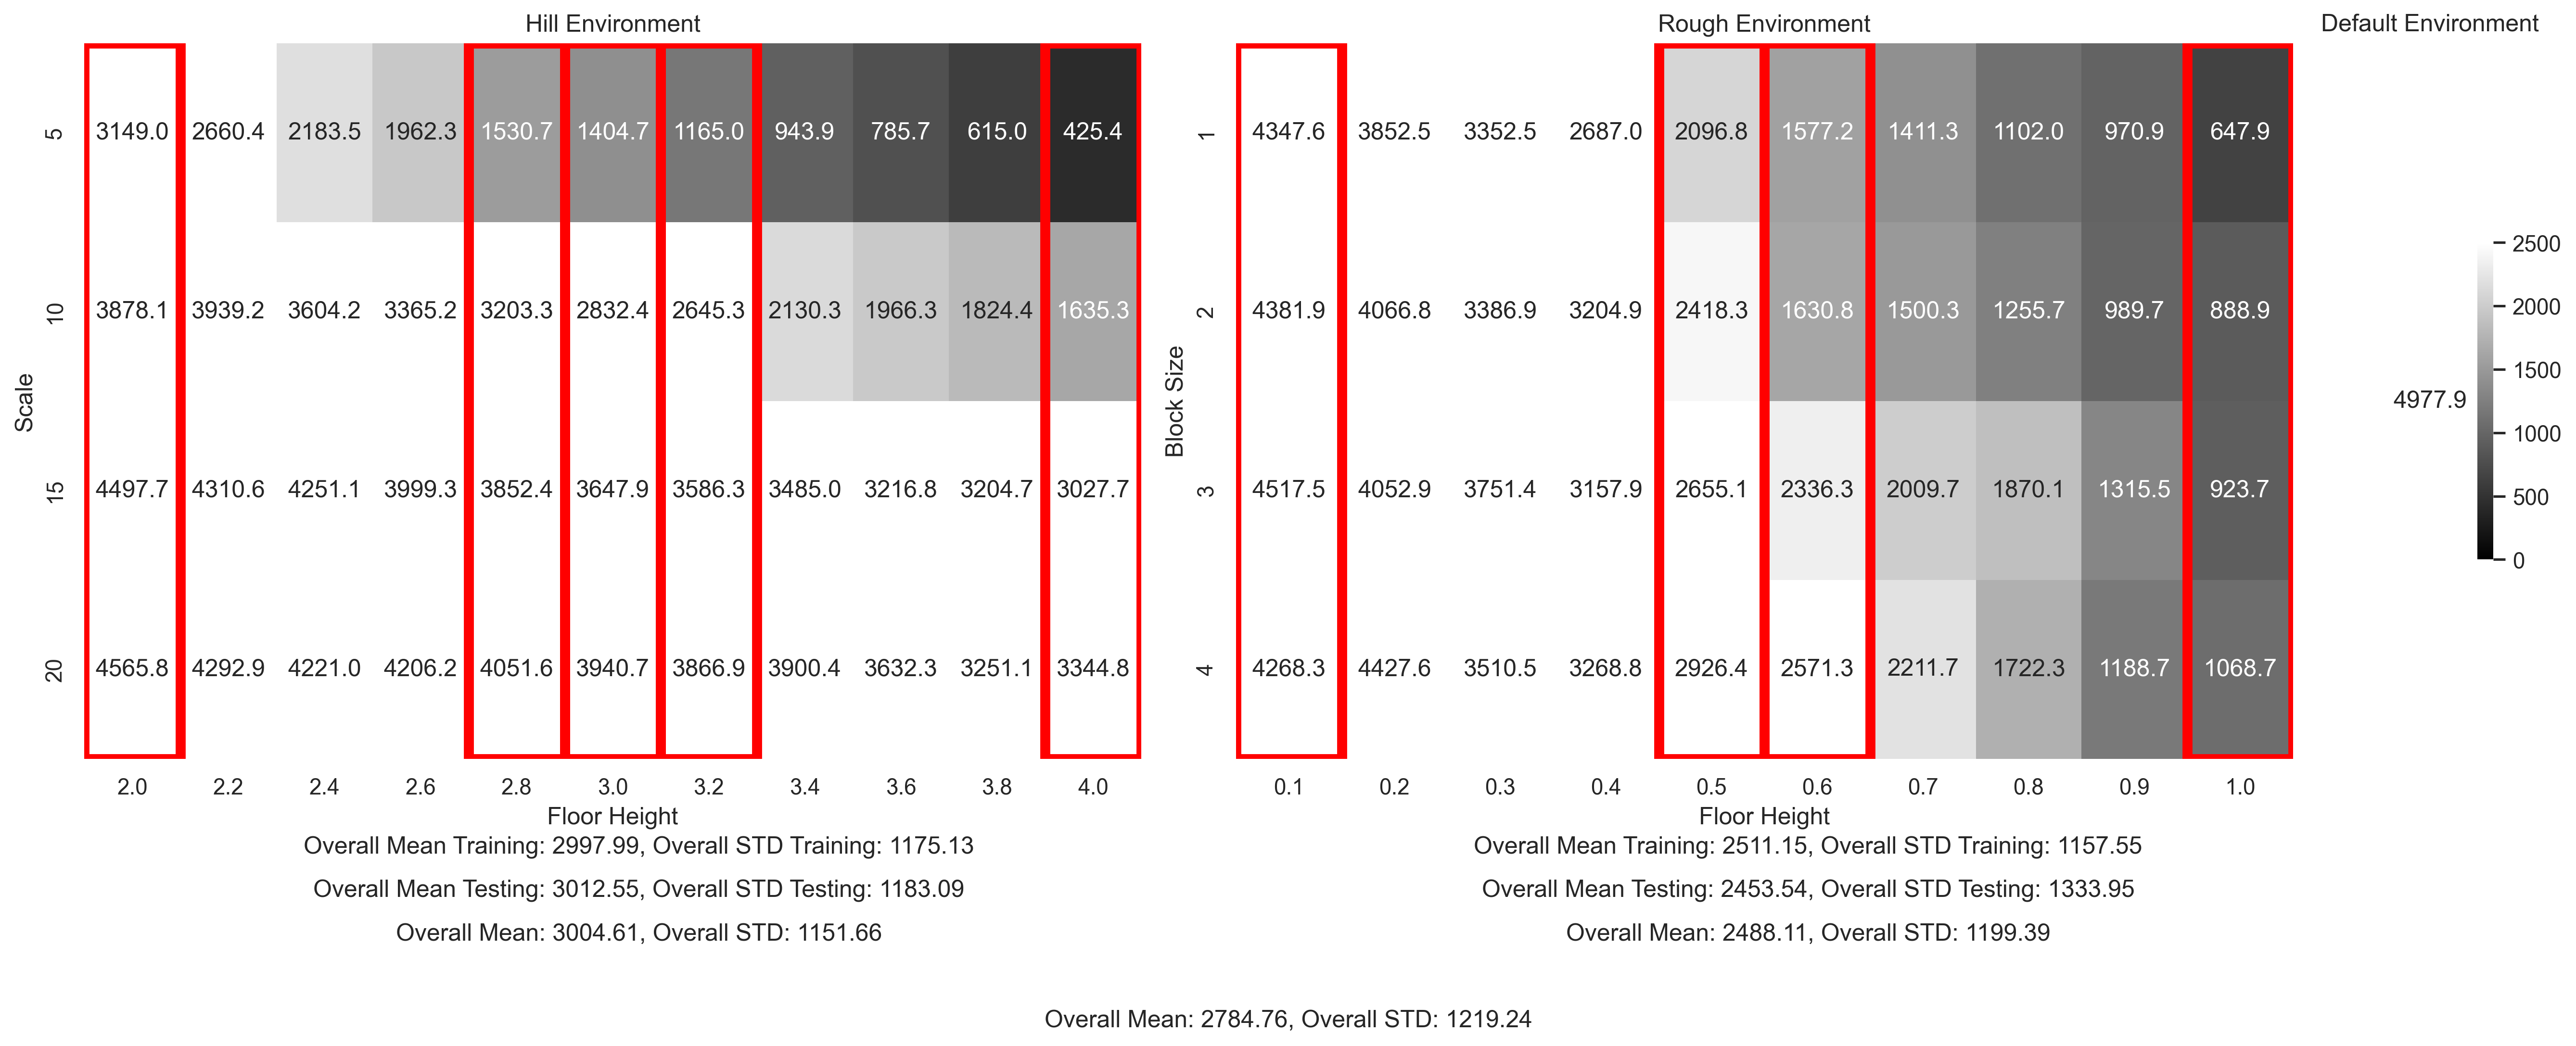
\includegraphics[width=\linewidth]{./resources/generalist_4_2784/fitness_heatmap.png}
            \caption{Experiment 1 - Fitness heatmap from one generalist MC-pair evolved over 5000 generations with partitions disabled}
            \label{fig:fit_heat_generalist}
        \end{figure*}

        Figure~\ref{fig:fit_heat_generalist} shows the obtained fitness scores for each environment, represented in a heatmap for experiment 1. For the hill environment, the heatmap shows high performance in the environments at the lower left and relatively lower performance when nearing the the upper right. This may indicate inherint complexity in certain environments compared to others. The fitness scores and their standard deviations on the training and testing sets are similar. The training set has a mean fitness score of 2997.99 with a standard deviation of 1175.13, and the testing set has a mean fitness score of 3012.55 with a standard deviation of 1183.09. 
        
        For rough terrain environment, the heatmap also shows high performance in the environments at the lower left and relatively lower performance when nearing the upper right, but also more at the lower right part. The fitness scores and their standard deviations on the training and testing sets are also similar. The training set has a mean fitness score of 2511.15 with a standard deviation of 1157.55, and the testing set has a mean fitness score of 2453.54 with a standard deviation of 1333.95.
    
        \subsection{Experiment 2: Partitioned generalist}
            \begin{figure*}[ht]
                \centering
                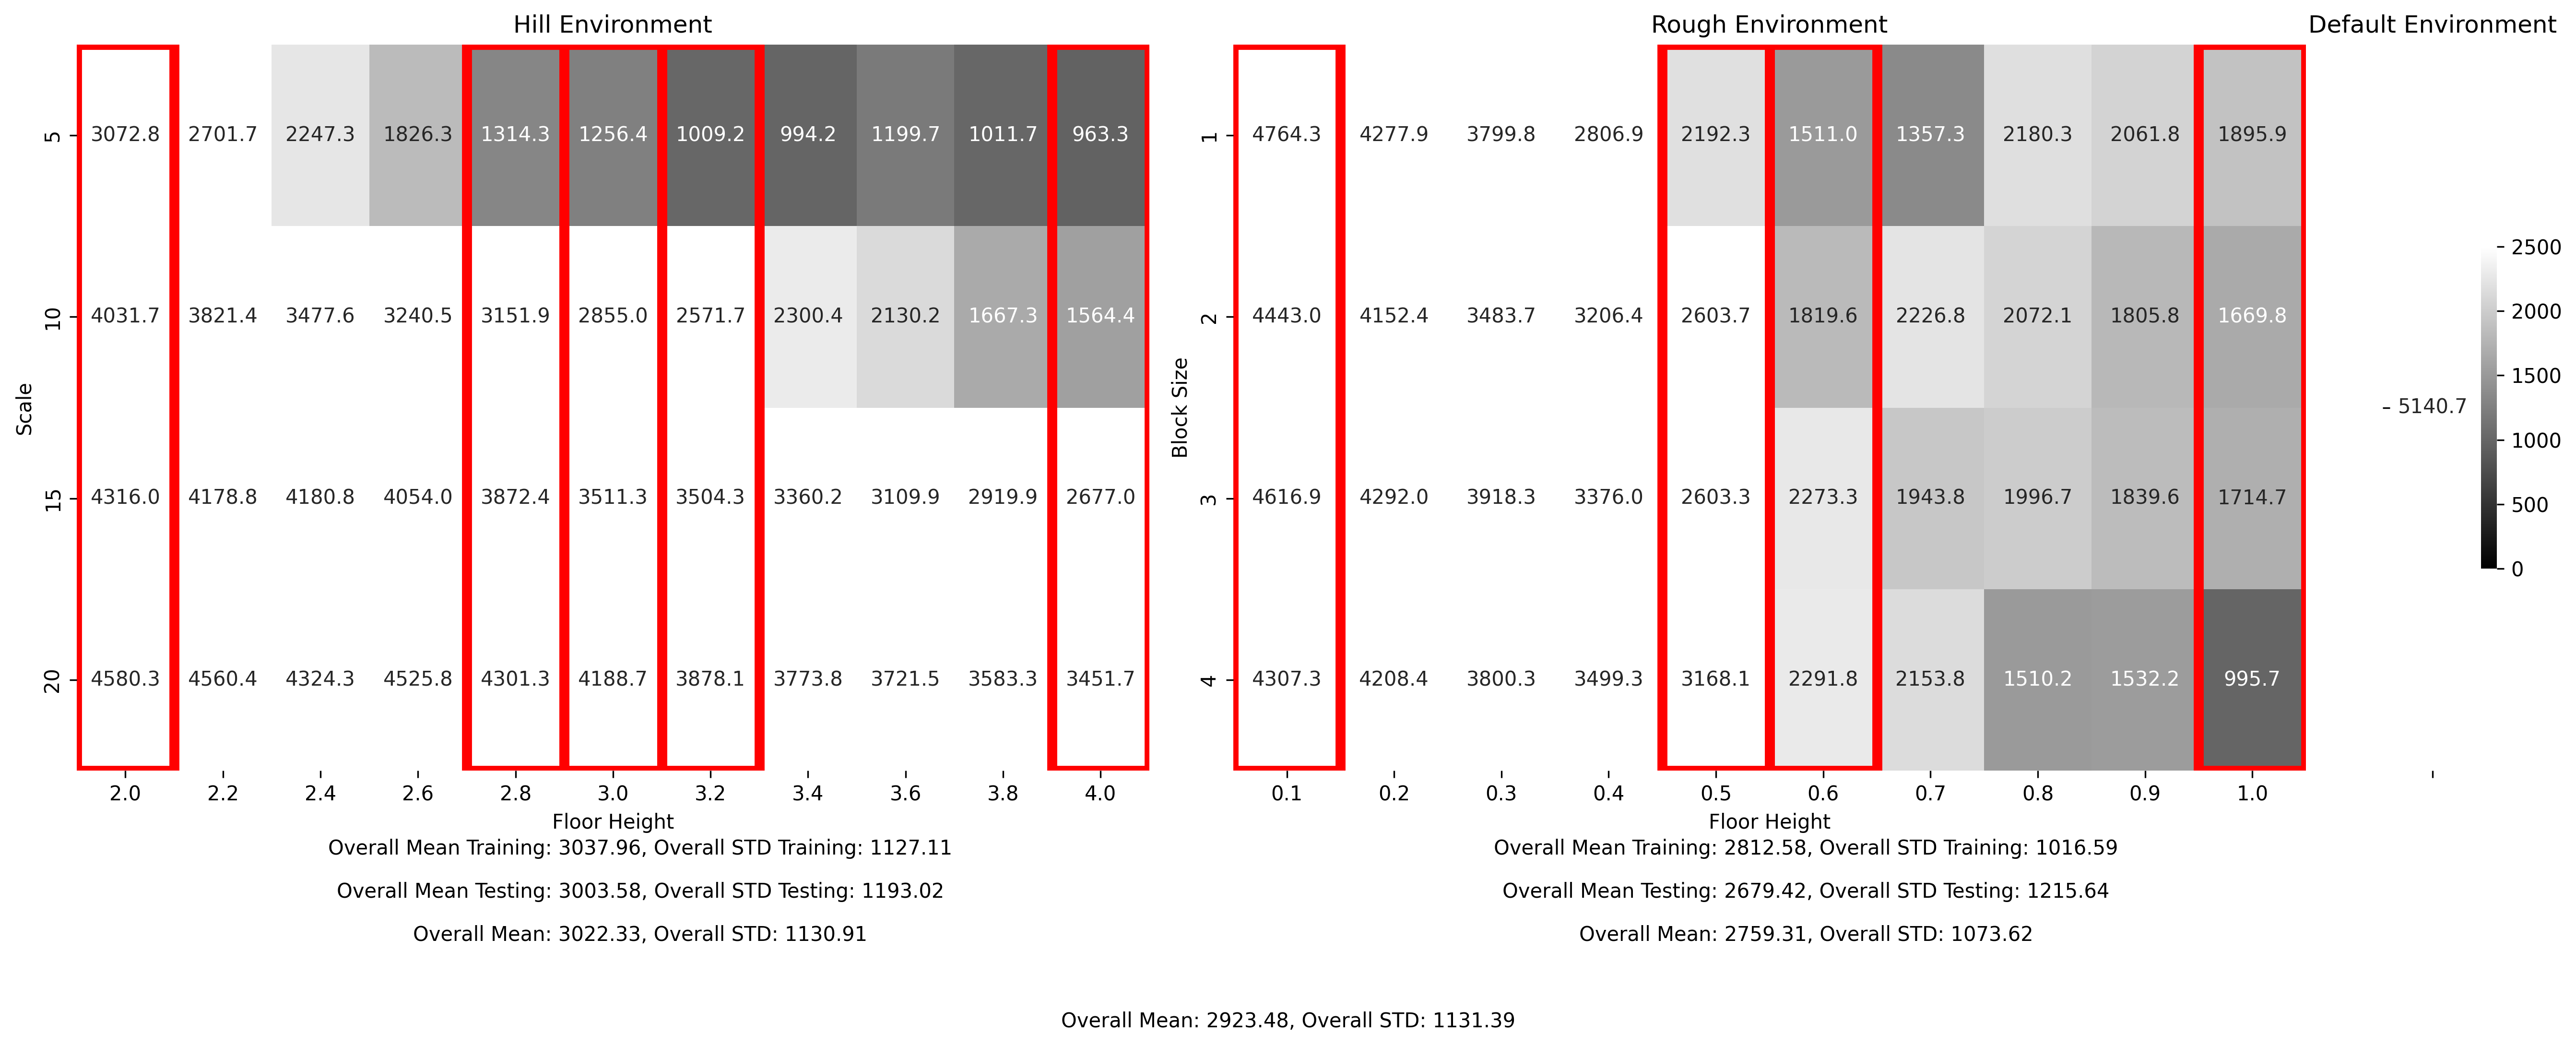
\includegraphics[width=\linewidth]{./resources/partition_5_2906_3/fitness_heatmap.png}
                \caption{Experiment 2 - Fitness heatmap of a set of generalist MC-pair}
                \label{fig:fit_heat_partitioned}
            \end{figure*}

            Figure~\ref{fig:fit_heat_partitioned} shows the obtained fitness scores for each environment, represented in a heatmap for experiment 2. For the hill environment, similar to experiment 1, the heatmap shows high performance in the environments at the lower left and relatively lower performance when nearing the the upper right. The fitness scores and their standard deviations on the training and testing sets are also similar. The training set has a mean fitness score of 3037.96 with a standard deviation of 1127.11, and the testing set has a mean fitness score of 3003.58 with a standard deviation of 1193.02. 

            For rough terrain environment, the heatmap also shows high performance in the environments at the lower left and relatively lower performance when nearing the upper right, but also more at the lower right part, similary as experiment 1. The fitness scores on the training and testing sets are slightly different. The training set has a mean fitness score of 2812.58 with a standard deviation of 1016.59, and the testing set has a mean fitness score of 2679.42 with a standard deviation of 1215.64. 
            
            \begin{figure*}[ht]
                \centering
                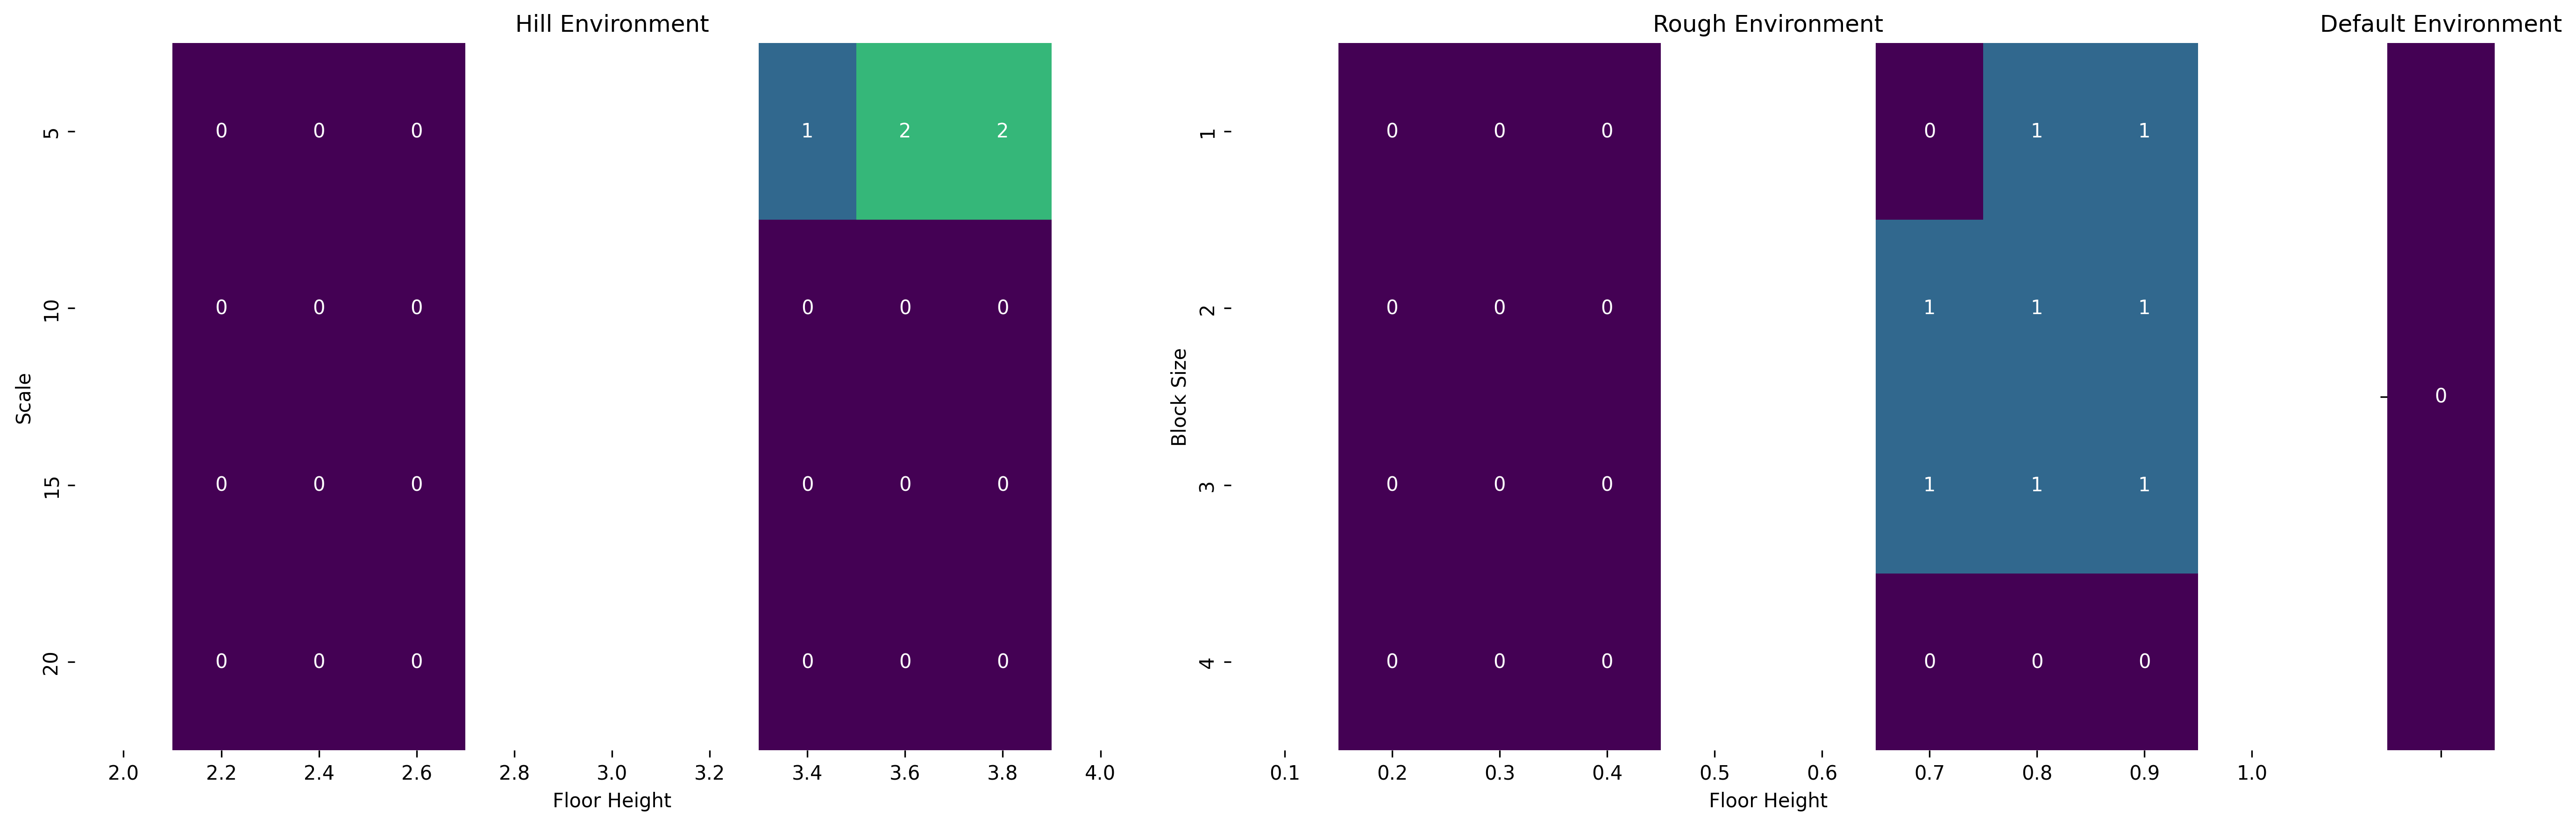
\includegraphics[width=\linewidth]{./resources/partition_5_2906_3/generalist_heatmap_partition.png}
                \caption{Experiment 2 - Figure showing to which partition the environment belongs to. In this experiment, three partitions where created.}
                \label{fig:heat_partition_number}
            \end{figure*}

            However, overall it does score a higher fitness score on the rough terrain environment compared to experiment one. This does make sense when looking at the partitions the algorithm took visible in figure~\ref{fig:heat_partition_number}. This figure shows the partition that the environment is assigned to. The blank white areas are the testing environments and are not assigned to a partition. In this experiment, the environments where partition one is handling the environment are of higher fitness scores, than in experiment one.

        \subsection{Experiment 3: Specialist for each environment}
